\section{Result: Reward network} \label{s:N_II:rwd}

% Introducing the reward
The reward network constructed following the pipeline in \cref{s:N_II:methods} uses the sigmoid modifier to reward the genes that are mutated. Compared to the standard network, the correlations (or nodes' weights) of mutated genes are increased proportionally with the mutation burden from TCGA's MIBC cohort. 


\begin{figure}[H]    
    \centering
    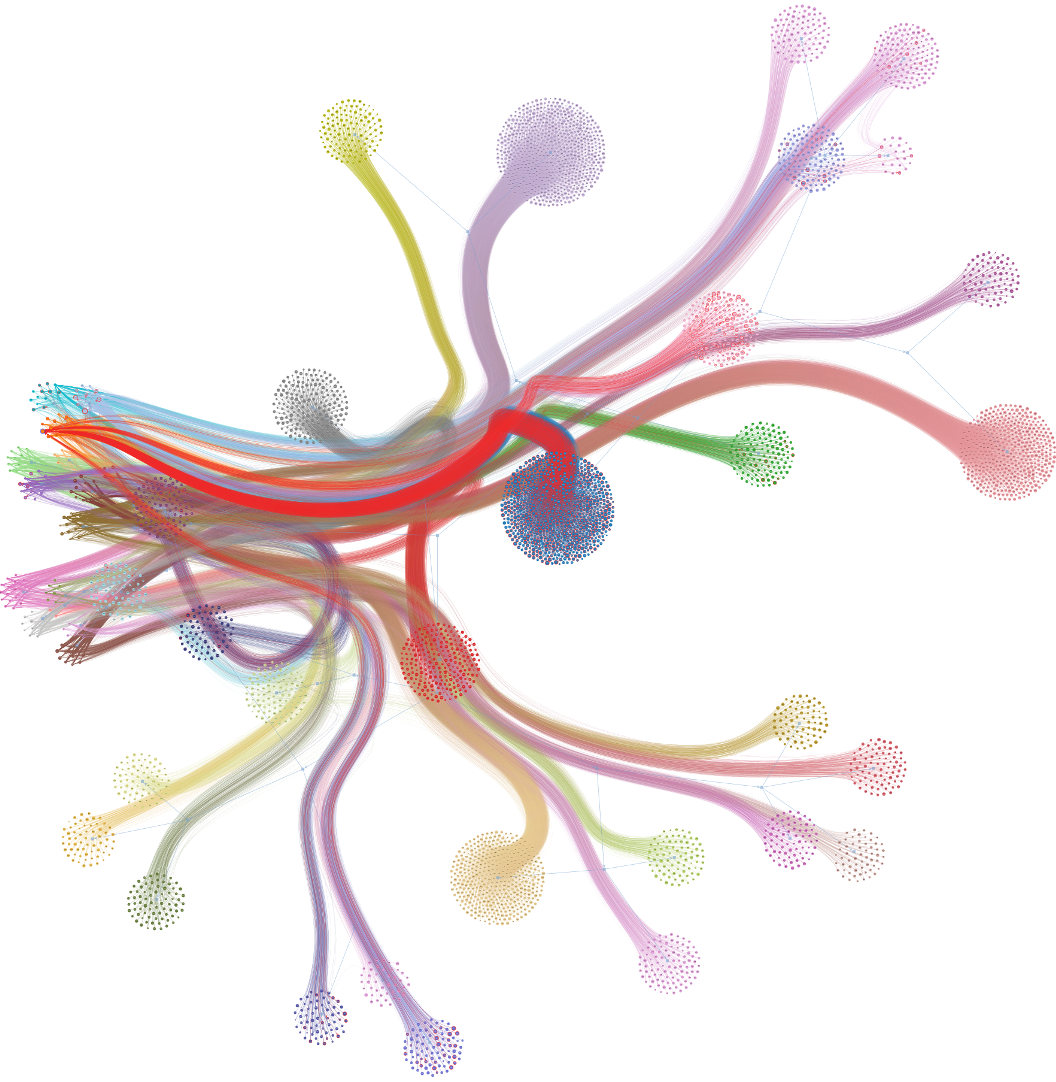
\includegraphics[width=1.0\textwidth,height=1.0\textheight,keepaspectratio]{Sections/Network_II/resources/reward/sigmoid_5K_AHR_sfdp.png}
    \caption{The reward network constructed from the 5000 most relatively varied genes, 3 edges per standard and 6 for TF, hierarchical SBM is used for community detection. The connections in red represents the the edges between \textit{AHR} and other genes, showing the importance of the gene in the network.}
    \label{fig:N_II:reward_net}
\end{figure}

% Describe the network 
% - small and large communities
The resultant network is shown in \cref{fig:N_II:reward_net} where it can be observed that there are is large variation in the community sizes. On the left hand side there is a group of small communities, while on the other side there are larger blocks of nodes such as community 0 (blue) or purple (\textbf{100}) at top. The imbalance between the community sizes was evident from the network metrics the standard vs. reward comparison in \cref{fig:N_II:net_metric_sig_std}, where the metrics suggested that the modified network contains nodes that are highly connected.

% Talk about the aspects of the networks
The red-lines are the edges from the \textit{AHR} gene to its neighbours gene which are mostly grouped in the largest community, 0. It was also observed that it is usually the case that smaller communities have genes that have a high degree and most of the edges lead to the larger communities. The genes in the large blocks (e.g., 0 or \textbf{100}) are not connected with each other but these nodes seems to be grouped by their links to the genes in the smaller communities; like community \textbf{101} of which \textit{AHR} is part of. 


\subsubsection*{Highly connected genes} \label{s:N_II:high_conn}

% Present the figure
To further understand the relationship between the size of a community (Y-axis) and nodes' degree (mean values on X-axis) the two metrics were plotted on a scatter plot in \cref{fig:N_II:largeSmall_com}. The markers sizes in the figure are proportional to their mean mutation burden, larger the point is the larger is the average of highly mutated genes across the TCGA. A community is label as a "HighDegree" when the mean degree is in the 70th percentile, while "LowDegree" otherwise. 

\begin{figure}[!htb]    
    \centering
    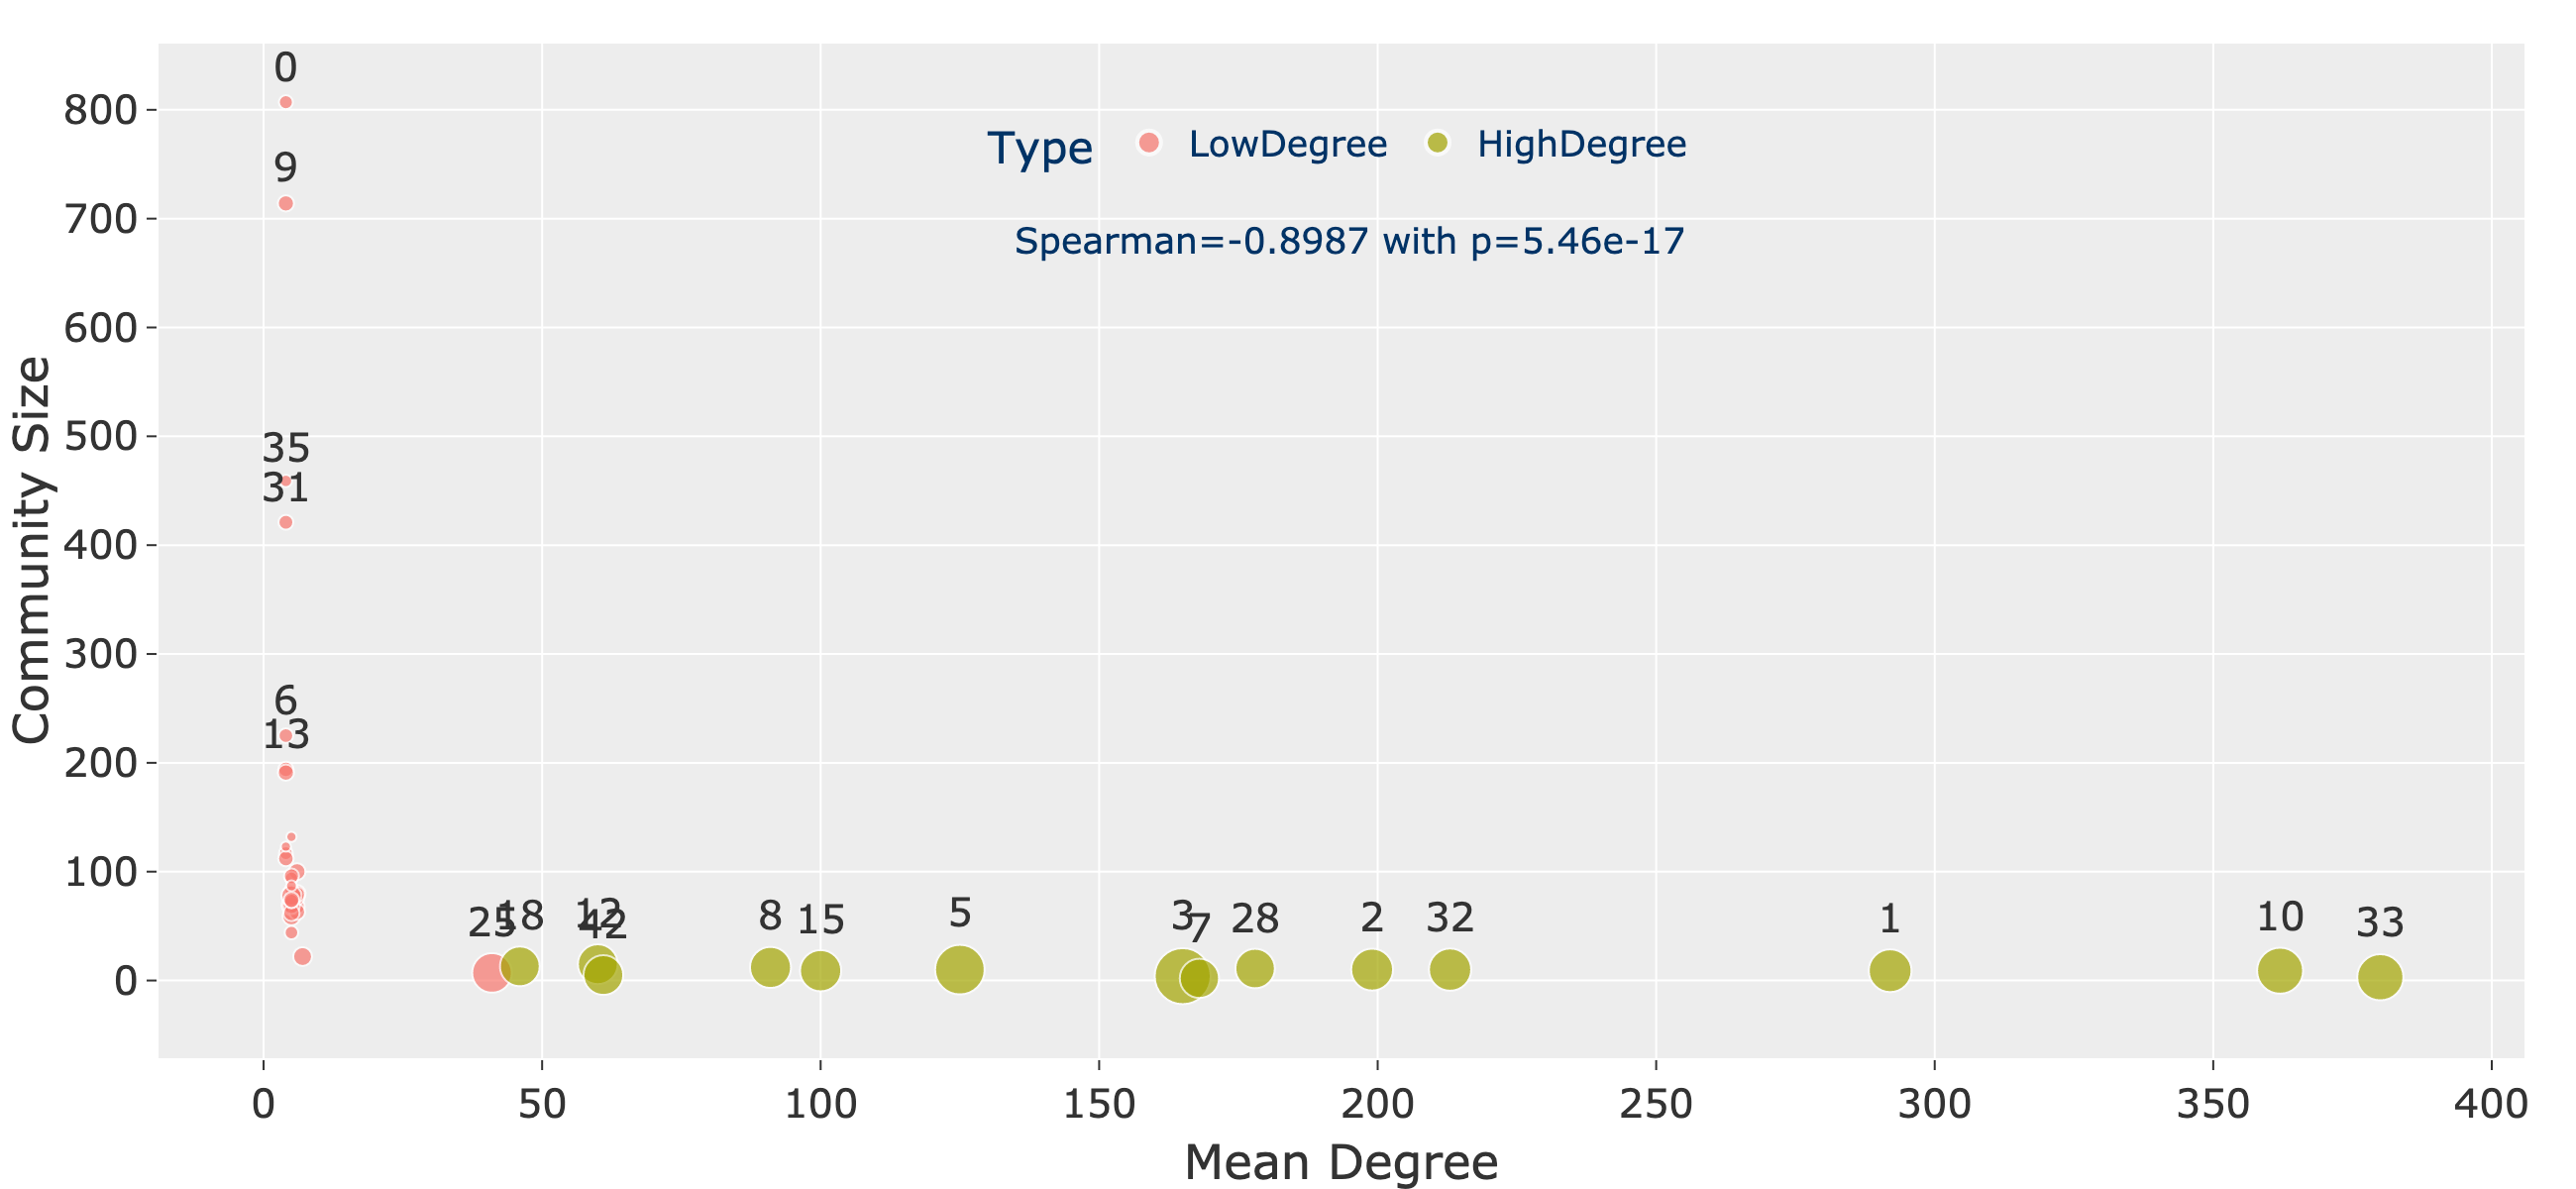
\includegraphics[width=1.0\textwidth,height=1.0\textheight,keepaspectratio]{Sections/Network_II/resources/reward/LargeSmall_com.png}
    \caption{Scatter plot showing the mean degree vs size of the communities found in the reward network. The marker size is proportional to the mean mutation burden in a community. The blocks are classified in two: 'HighDegree' which consists of the communities that have a mean degree in the top 30\% and "LowDegree' the rest of the blocks. Ii can be seen that there is a direct correlation of community size and mean degree.}
    \label{fig:N_II:largeSmall_com}
\end{figure}

% Interpret the figure
By having the communities with high connected genes close to the the X-axis and the other type close to the Y-axis, it indicates the relationship between the group size and degree. This is further confirmed by the negative Spearman correlation shown on the plot with $\rho=-0.8987$ with a $p=5.46e^{-17}$. The positive correlation between the community size and the average mutation count in a group highlights that the well-connected communities have a high mutation burden.

% Implication of the finding
This initial analysis shows the \acrfull{hsbm} separately groups the mutated genes with a high degree from the rest of the nodes. This indicates that the community detection is capable of finding very small communities of just a few nodes from the 5000 genes used to build the network. In addition, the un-connected genes can be grouped together in larger blocks. 

% talk about the source of this imbalance around the communities
These two observations attest the power of the community detection but it does not explain the size imbalance across communities. The genes that are in small and well-connected communities tend to have a high correlation even in an un-modified network (\textbf{How can I show this}). The selective edge pruning keeps only the 3 or 6 top most correlated genes which is the reason nodes like \textit{AHR} do not have a higher degree in the standard network. As the sigmoid modifier increases the correlation values of mutated genes, the genes which have a reasonable high correlation but they are not in the top selected genes. 

% Example for AHR 
For example, \textit{AHR} is a mutated gene which is also correlated with the expression of other genes. \textit{AHR} is allowed only 3 or 6 connections, the rest of the connections need to come from the 'other genes'. In the standard network, \textit{AHR} is not in the top correlated values of these 'other genes', but as the sigmoid modifier the \textit{AHR} is pushed in the top. Thus, leading for \textit{AHR} to have a higher degree. This examples illustrated how the weight modifier and the community detection groups these highly connected nodes.




\begin{figure}[!htb]    
    \centering
    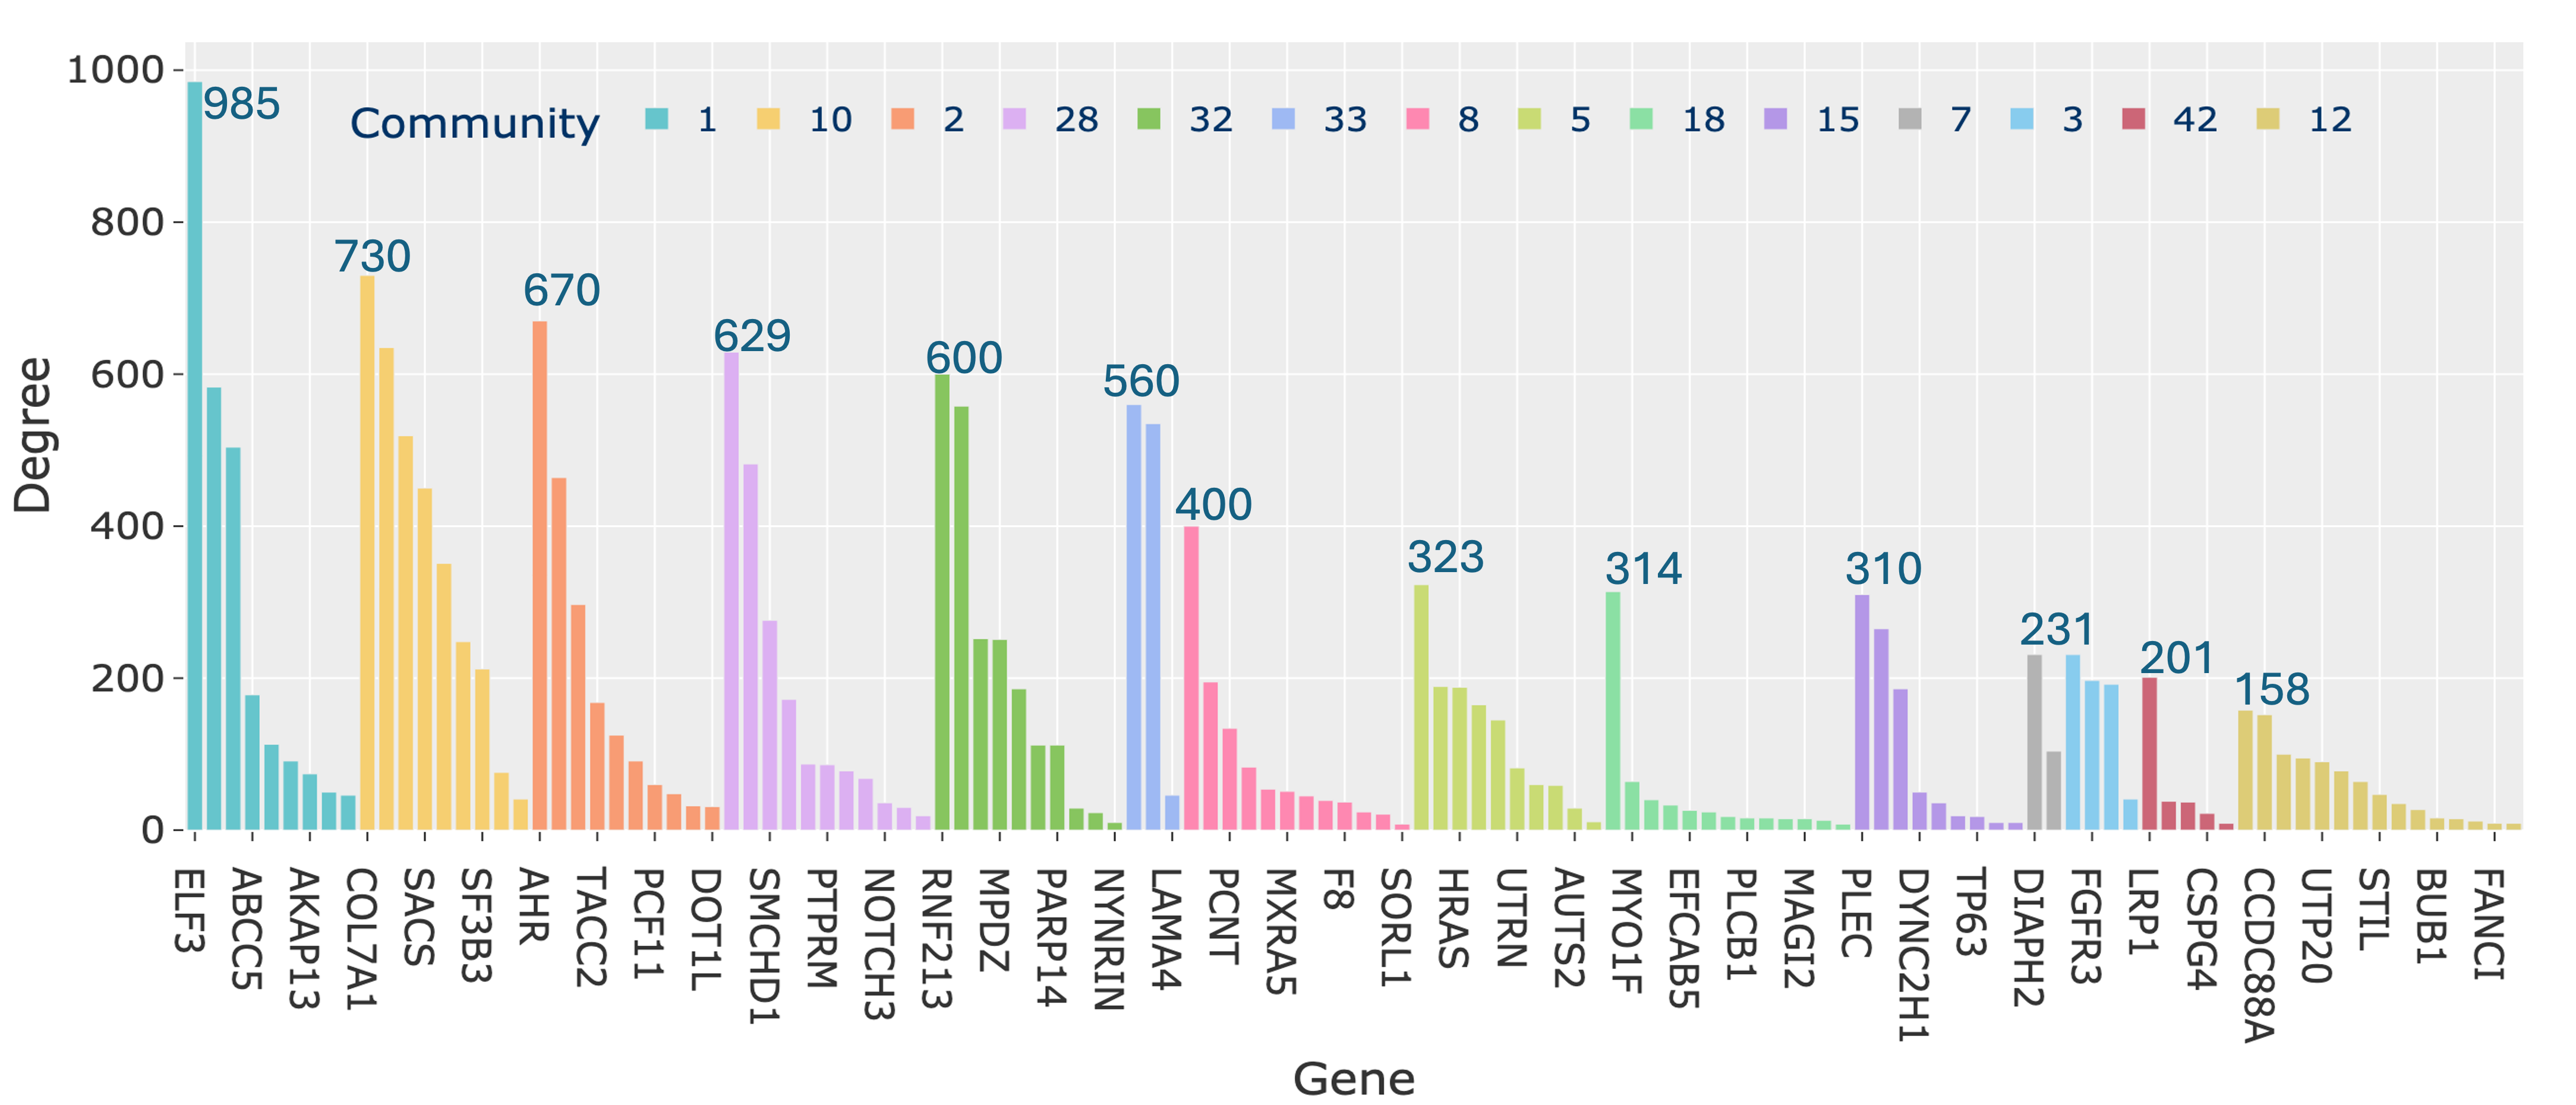
\includegraphics[width=1.0\textwidth,height=1.0\textheight,keepaspectratio]{Sections/Network_II/resources/reward/SmallCom_gene_labeled.png}
    \caption{Mean degree vs size}
    \label{fig:N_II:genes_highConn}
\end{figure}



\subsection{AHR search}

\subsection{PPARG and RARG}

\subsection{Low connected}

\subsection{Comparison with Standard Network}